
\chapter{Desenvolvimento}\label{desenvolvimento}

\section{Etapas}\label{etapas}

\subsection{Aquisição dos dados}\label{aquisicao-dos-dados}

\subsubsection{Área de Estudo}\label{area-de-estudo}

Primeiro foi feito o \emph{download} de um arquivo no
formato \emph{shapefile}, da malha territorial do estado de São Paulo,
com divisão por município, disponibilizado pelo \sigla{IBGE}{Instituto Brasileiro de Geografia e Estatística} \cite{ibge-malha}. A partir desse arquivo, foi selecionado apenas o polígono que representa o município de Bauru. A biblioteca no R utilizada para tal operação foi a \textit{sf} \cite{sf}.

\subsubsection{Imagens de Satélite}\label{imagens-de-satelite}

Os dados do sensor Sentinel-2/MSI podem ser obtidos gratuitamente, mediante apenas a um cadastro realizado no \textit{Copernicus Open Access Hub} \cite{sentinel-data}. No R, há diversas bibliotecas que fazem a interface com a API do \textit{hub}, para este trabalho foi escholhida a \textit{getSpatialData} \cite{getSpatialData}. 
    
    O sensor multiespectral do Sentinel-2 possui as características descritas na \autoref{t.sentinel-msi}.

\begin{table}[ht]
\centering
\caption{Características das bandas do sensor multiespectral MSI do Satélite Sentinel-2}
\begin{tabular}{rllrr}
  \hline
 banda & nome & lambda & resolucao \\ 
  \hline
 B1 & Aerosol & 0.44 &  60 \\ 
 B2 & Azul & 0.49 &  10 \\ 
 B3 & Verde & 0.56 &  10 \\ 
 B4 & Vermelho & 0.67 &  10 \\ 
 B8 & NIR & 0.84 &  10 \\ 
 B5 & Red edge 1 & 0.70 &  20 \\ 
 B6 & Red edge 2 & 0.74 &  20 \\ 
 B7 & Red edge 3 & 0.78 &  20 \\ 
 B9 & Vapor d’água & 0.94 &  60 \\ 
 B10 & Cirrus & 1.38 &  60 \\ 
 B11 & SWIR 1 & 1.61 &  20 \\ 
 B12 & SWIR 2 & 2.19 &  20 \\ 
 B8A & Red edge 4 & 0.86 &  20 \\ 
   \hline
\end{tabular}
\label{t.sentinel-msi}
\legend{Fonte: Elaborado pelo autor}
\end{table}

A partir dos filtros por data e cobertura de nuvem, foram selecionadas duas imagens e então realizada uma composição entre elas para que recobrissem a área de interesse completamente. Posteriormente, foi feito um redimensionamento das bandas de 20m para 10m, para que fossem compiladas em uma única pilha de \textit{raster}. Selecionando as bandas B04, B03 E B02, é possível visualizar a imagem nas cores vermelho, verde e azul, respectivamente, como visto na \autoref{fig-rgb}. A biblioteca utilizada que manipula arquivos \textit{raster} no R é a \textit{raster} \cite{raster}.

% \begin{figure}[htbp]
\begin{figure}[H]
    \centering
    \caption{Composição com as bandas vermelha, verde e azul do Sentinel-2/MSI para a região da região do município de Bauru} \label{fig-rgb}
    \includegraphics[scale=0.55]{figs/plot_sentinel-rgb.pdf}
    \legend{Fonte: Elaborado pelo autor}
\end{figure}

\subsubsection{Seleção de Amostras}\label{selecao-de-amostras}

    Para a seleção das amostras de treinamento, era preciso que os dados
representassem bem as classes de uso e cobertura do solo dentro do
município. De acordo com o SEMMA (2015) e CAVASSAN (2013), as principais unidades fitogeográficas que ocorrem no município de bauru são as formações de Floresta Estacional Semidecidual e de Cerrado, apesar de a cobertura primitiva já tenha sido muito reduzida, assim como o Cerrado no estado de São Paulo, que já representou uma área maior.

    Portanto, duas decisões foram tomadas: as amostras de treinamento
seriam provindas do bioma Cerrado; como a extensão o Cerrado é grande, a
fim de viabilizar o processamento, apenas a região de cerrado dentro do
estado de São Paulo foi selecionada.

	Para isso, foi utilizado um \textit{raster} da coleção 3.1 do projeto MapBiomas \cite{mapbiomas2018coleccao} contendo os valores de cada classe para cada pixel, definidos pela metodologia aplicada pelo projeto. As classes utilizadas estão referenciadas na Tabela 2.

\begin{table}[H]
\legend{Fonte: Elaborado pelo autor}
\label{tab-classes}
\centering
\caption{Classes de uso e cobertura da terra da coleção 3.1 do MapBiomas para o bioma Cerrado}
\begin{tabular}{rrl}
  \hline
 value & name.full \\ 
  \hline
 3 &         1.1.1. Formação Florestal \\ 
4 &         1.1.2. Formação Savanica \\ 
   9 &     1.2. Floresta Plantada \\ 
  12 &     2.2. Formação Campestre \\ 
  15 &     3.1. Pastagem \\ 
  19 &          3.2.1. Cultura Anual e Perene \\ 
  20 &          3.2.2. Cultura Semi-Perene \\ 
  21 &     3.3. Mosaico de Agricultura e Pastagem \\ 
  24 &     4.2. Infraestrutura Urbana \\ 
  33 &     5.1 Rio, Lago e Oceano \\ 
   \hline
\end{tabular}
\legend{Fonte: Elaborado pelo autor}
\end{table}

    Esse \emph{raster} foi recortado para o tamanho do polígono do estado
de São Paulo. Em seguida, foi feito a seleção de duzentas amostras aleatórias
de cada classe, representadas na Figura 3, e em seguida foi exportado para um arquivo \emph{shapefile}.

\begin{figure}[H]
    \label{fig-amostras}
    \centering
    \caption{Amostras aleatórias de pontos contidos na região de cerrado do Estado de São Paulo}
    \includegraphics[scale=0.6]{figs/plot_pontos-amostra.pdf}
    \legend{Fonte: Elaborado pelo autor}
\end{figure}

\subsection{Extração de
Características}\label{extracao-de-caracteristicas}

	A etapa da extração de características envolve a seleção das variáveis
usadas no processo de classificação, que podem ser as assinaturas
espectrais das bandas, índices de vegetação, informação de textura,
entre outras \cite{lu-weng}

\subsubsection{Extração dos Valores das
Amostras}\label{extracao-dos-valores-das-amostras}

    A próxima etapa, foi a de extração dos valores das amostras. Cada
coordenada gerada na última etapa, contém a informação da classe que ela representa, então o próximo passo foi de extrair os valores de cada
banda naquele ponto, e então compor a tabela com as variáveis preditoras
para a modelagem de aprendizado de máquina.

    Nessa etapa, foi utilizado o ambiente do \textit{Google Earth Engine} \cite{gorelick2017google} , onde o \emph{shapefile} foi carregado, foi feita uma composição com imagens do satélite Sentinel-2, filtradas por baixa porcentagem de nuvens e para a região em que os pontos estão compreendidos. Em seguida, para cada ponto, foi extraído os valores das bandas, como mostra a Tabela 3, e exportado para um arquivo \emph{geojson}, que foi importado de volta ao ambiente do RStudio.
    
\begin{table}[H]
    \label{tab.freq}
    \caption{Quantidade de exemplos de treinamento para cada classe}
  	\centering
  	\begin{tabular}{rlr}
    	\hline
   		& Classes & Frequência \\ 
    	\hline
  	1 & agricultura\_pastagem & 197 \\ 
    2 & cultura\_anual\_perene & 146 \\ 
    3 & cultura\_semi\_perene & 200 \\ 
    4 & floresta\_plantada & 200 \\ 
    5 & formacao\_campestre & 140 \\ 
    6 & formacao\_florestal & 199 \\ 
    7 & formacao\_savanica &  91 \\ 
    8 & infra\_urbana & 105 \\ 
    9 & pastagem & 198 \\ 
    10 & rio\_lago\_oceano & 159 \\ 
    	\hline
	\end{tabular}
	\legend{Fonte: Elaborado pelo autor}
\end{table}

É importante notar que para algumas classes, na execução da amostragem, foram selecionados menos do que duzentas amostras, pois haviam poucos pixels representantes. 

    Em um sistema de classificação, antes da extração dos valores dos pontos das amostras, seria interessante que a imagem passasse por um
processo de pré processamento. Essa etapa incluiria a aplicação de
técnicas de processamento de imagens para correções atmosféricas e
geométricas, eliminação de ruídos, entre outras \cite{lu-weng}. Contudo, uma característica das imagens do Sentinel-2/MSI, é de que há uma série de etapas de pré processamento, como as mencionadas, que são realizadas antes das imagens serem disponibilizadas. 

\subsubsection{Índices de
Vegetação}\label{indices-de-vegetacao}

	Os índices de vegetação são obtidos através de operações aritméticas
entre as bandas. Possuem a característica de realçar as variações de
densidade da cobertura vegetal \cite{meneses2012introduccao}. O NDVI é provavelmente o mais utilizado, ou pelo menos o mais conhecido. Esse índice possui a característica de evidenciar áreas da vegetação fotossinteticamente mais ativas. O cálculo do NDVI, que varia de 0 a 1, é dado por: 

\begin{equation}
NDVI = \frac{NIR - RED}{NIR + RED}
\end{equation}

Onde $NIR$ é o valor para a banda na região do infravermelho próximo
(a banda 8 do Sentinel-2/MSI) e $RED$ é a banda na região do vermelho (banda 4). A Figura 4 mostra uma representação do cálculo do \acs{NDVI}.

\begin{figure}[H]
    \centering
    \caption{Representação do cálculo do índice NDVI} \label{fig-fluxograma}
    \includegraphics[scale=0.7]{figs/plot_ndvi.pdf}
    \legend{Fonte: Elaborado pelo autor}
\end{figure}

\subsubsection{Seleção de Variáveis}\label{selecao-de-variaveis}

	Como variáveis preditoras, foram selecionadas as bandas ``SWIR1'',
``SWIR2'', ``Azul'', ``Verde'', ``Vermelho'', ``NIR'', ``RE1'', ``RE2'',
``RE3'', ``RE4'' e uma nova coluna contendo o cálculo do NDVI para cada
ponto da amostra.


\subsection{Modelagem}\label{modelagem}

	O pacote \emph{caret} (\emph{Classification And REgression Training}) \cite{caret} R contém funções para otimizar o processo de treinamento de modelos para problemas de regressão e classificação. Ele funciona como um agregador de diversos pacotes que contém métodos de aprendizado estatístico, fazendo a interface entre as funções disponíveis no pacote para controle do processo de treinamento e avaliação de resultados.

\subsubsection{Reamostragem}\label{reamostragem}

	A primeira etapa para a criação dos modelos, foi a divisão do conjunto
de dados em dois subconjuntos: um de treinamento (75\%) e outro de teste (25\%). Utilizando a função de validação cruzada do \emph{caret}, na criação do modelo, o conjunto de treinamento é reparticionado em 10, e então, a partir dessa repetições no ajuste, é escolhido o conjunto de
parâmetros que teve melhor resultado para aquele método.

\subsubsection{Treinamento}\label{treinamento}

	Na etapa do treinamento dos modelos, para a seleção dos parâmetros
utilizados em cada algoritmo foi utilizada a técnica da validação
cruzada \emph{k-fold} (não é o mesmo que na última etapa), onde os dados de treinamento são subdivididos em \emph{k} subconjuntos e então, o modelo é calculado \emph{k} vezes, e então, o resultado é comparado para seleção do parâmetro (ou conjunto) que obteve melhor resultado, no caso, o método de comparação utilizado foi a acurácia geral a partir da matriz de confusão gerada para cada modelo, como mostra a Figura 5, Figura 6 e Figura 7.

	O primeiro modelo foi treinado com o algoritmo MVS (\emph{svmRadial} no \emph{caret}), utilizado como núcleo a função de base radial dada por: 
    \begin{equation}
	K(x,y) = \exp(-\frac{\parallel x-y^{2} \parallel}{\sigma^{2}})    
    \end{equation}
	Após o treinamento do modelo, foram selecionados os parâmetros $C = 1$ e $Sigma = 1$.
    
\begin{figure}[H]
    \centering
    \caption{Parâmetros selecionados após treinamento com o algoritmo maquina de vetores suporte com núcleo radial} \label{fig-fluxograma}
    \includegraphics[scale=0.5]{figs/plot_svm-radial.pdf}
    \legend{Fonte: Elaborado pelo autor}
\end{figure}

	O próximo modelo, foi MVS também, porém linear (\emph{svmLinear3} no
\emph{caret}), ou seja, sem função de núcleo e com regularização, que
significa aplicar um custo de penalização nos parâmetros $\theta$. Os
parâmetros selecionados foram C = 0.03 e Loss = L2.

\begin{figure}[H]
    \centering
    \caption{Parâmetros selecionados após treinamento com o algoritmo maquina de vetores suporte linear com regularização} \label{fig-fluxograma}
    \includegraphics[scale=0.5]{figs/plot_svm-linear.pdf}
    \legend{Fonte: Elaborado pelo autor}
\end{figure}

	Por último, foi computado também um modelo utilizando Florestas
Aleatórias (\emph{rf} no \emph{caret}), com o parâmetro selecionado mtry
= 3.

\begin{figure}[H]
    \centering
    \caption{Parâmetros selecionados após treinamento com o algoritmo florestas aleatórias} 
    \includegraphics[scale=0.5]{figs/plot_rf.pdf}
    \legend{Fonte: Elaborado pelo autor}
\end{figure}

\section{Resultados}\label{resultados}

\subsection{Predição dos Dados}\label{predicao-dos-dados}

	Para cada modelo treinado, foi realizada uma predição com a imagem
selecionada anteriormente do sensor  Sentinel-2/MSI para a região do
município de Bauru, resultando em \emph{rasters} com os valores para
cada classes usadas para a criação dos modelos, demonstrados na Figura 8, Figura 9 e Figura 10.

\begin{figure}[H]
    \centering
    \caption{Mapa com classes de uso e cobertura da terra obtido a partir da predição do modelo utilizando MVS com núcleo radial} 
    \includegraphics[scale=0.8]{figs/map_svm-radial.pdf}
    \legend{Fonte: Elaborado pelo autor}
\end{figure}
\begin{figure}[H]
    \centering
    \caption{Mapa com classes de uso e cobertura da terra obtido a partir da predição do modelo utilizando MVS linear com regularização} 
    \includegraphics[scale=0.8]{figs/map_svm-linear.pdf}
    \legend{Fonte: Elaborado pelo autor}
\end{figure}
\begin{figure}[H]
    \centering
    \caption{Mapa com classes de uso e cobertura da terra obtido a partir da predição do modelo utilizando FA's} 
    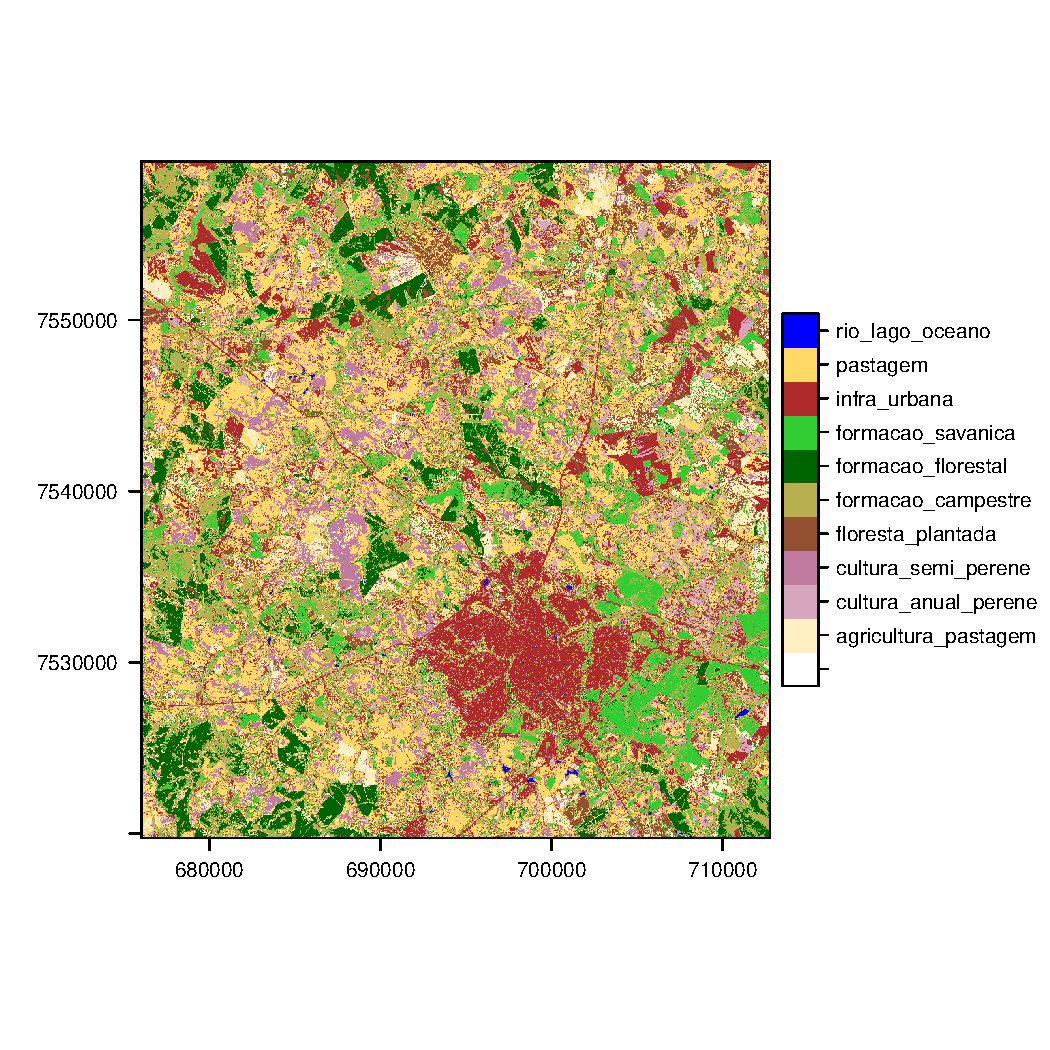
\includegraphics[scale=0.8]{figs/map_rf.pdf}
    \legend{Fonte: Elaborado pelo autor}
\end{figure}

\subsubsection{Avaliação de
Precisão}\label{avaliacao-de-precisao}

Para a avaliação da qualidade das predições realizadas, foi computado
a matriz de confusão de cada uma, a partir dos índices calculados a
partir da matriz de erro. A matriz de erro por sua vez foi montada a
partir da seleção de 100 pontos de amostras para cada classe dos
\emph{rasters} obtidos na etapa da predição, e em seguida, os valores
dos pontos foram extraídos de um conjunto verdade, que é um
\emph{raster} da mesma região com a classificação realizada pela
iniciativa MapBiomas e disponibilizada para download. Para comparação
visual com os mapas apresentados anteriormente, o \emph{raster} do
MapBiomas está representado na Figura 11.

\begin{figure}[H]
    \centering
    \caption{Mapa com classes de uso e cobertura da terra obtido a partir da classificação realizada pela iniciativa MapBiomas} 
    \includegraphics[scale=0.8]{figs/map_mapbiomas.pdf}
    \legend{Fonte: Elaborado pelo autor}
\end{figure}

Com destaque para os índices \emph{kappa} e \emph{accuracy} (acurácia geral), na Tabela 4 a seguir estão demonstrados os valores dos resultados:

\begin{table}[H]
\caption{Tabela de avaliação de precisão das predições realizadas}
\centering
\begin{tabular}{rlrr}
  \hline
 & Modelo & Kappa & Acuracia \\ 
  \hline
1 & MVS linear & 0.30 & 0.38 \\ 
  2 & MVS radial & 0.27 & 0.39 \\ 
  3 & Florestas Aleatorias & 0.13 & 0.23 \\ 
   \hline
\end{tabular}
\end{table}

\subsubsection{Considerações}\label{considerauxe7uxf5es}

Comparando visualmente os mapas obtidos com o mapa do MapBiomas além da matriz de erro gerada, pôde-se notar algumas classes que sofreram certa confusão, como é o caso da \emph{formação\_florestal} na predição com FA, que na verdade representariam a classe \emph{floresta\_plantada}. Levando em consideração que na  metodologia do MapBiomas aplicada nos dados de
treinamento são utilizadas outras variáveis de predição (como outros
índices de vegetação), é provável que apenas as bandas selecionadas e o
NDVI não seja suficiente para separar com precisão todas as classes
utilizadas, como LU e WENG (2007) apontam no artigo o qual este trabalho se
baseou. Ainda no caso dessa predição, a acurácia foi prejudicada pelo
fato dos \emph{pixels} apresentarem pouca homogeneidade nos espaços
vizinhos. A predição realizada com o algoritmo MVS com núcleo não
linear, apesar de apresentar uma acurácia mediana, resultou em poucas
classes que predominaram. A classificação que obteve melhor resultado
foi a que utilizou MVS linear para criação do modelo.
